%allowed options finnish, swedish, english
%after changing the language you may be forced to use recompile from scratch to get rid of errors
\documentclass[finnish]{docopts}
\usepackage{epsfig}
\usepackage{subfigure}
\usepackage{url}
\usepackage{natbib}
\usepackage{tikz}
\usepackage{bm}
\usepackage{amsmath}
\usepackage{booktabs}



\begin{document}


%\doublespacing
%\onehalfspacing
\singlespacing

\title{Lineaarinen sekamalli rekisteripohjaisen lasten ja nuorten neuvola- ja kouluterveysaineiston analyysivälineenä}
\author{Petteri Mäntymaa}
\date{\today}

\maketitle

%\classification{\protect{\ \\
%\  Outline1 $\rightarrow$ Outline2 $\rightarrow$ Outline3\  \\
%\  Outline4 $\rightarrow$ Outline5 $\rightarrow$ Outline6 $\rightarrow$ Outline7\ }}

\keywords{avainsanat, avainsanat, avainsanat}

\begin{abstract}

TIIVISTELMÄ

\end{abstract}

\mytableofcontents

\section{Johdanto}


\section{Pitkittäistutkimus tutkimusasetelmana}

Pitkittäistutkimuksen määrittelevänä ominaispiirteenä pidetään yleisesti yhden tai useamman yksilön seurantaan perustuvaa asetelmaa, jossa samasta yksilöstä saadaan havaintoja eri aikoina \citep{diggle02, fitzmaurice11, twisk13, laird82}. Toistuvat havainnot samasta yksilöstä mahdollistavat ajassa tapahtuvien muutosten, muutokseen vaikuttaneiden tekijöiden, kuin myös yksilön yksilöllisistä ominaisuuksista koostuvien tekijöiden tunnistamisen ja analysoinnin.

\cite{diggle02} mukaan taloustieteessä ja yhteiskuntatieteissä voidaan pitkittäistutkimuksesta käyttää myös termiä paneelitutkimus, mutta sovellettujen tilastollisten menetelmien kannalta, erityisesti terveystieteellisissä ja epidemiologisissa tutkimuskysymyksissä, käsitteet \textit{pitkittäistutkimus} ja sen yhteydessä havaittu \textit{pitkittäisaineisto} muodostavat luontevamman viitekehyksen.

\cite{twisk13} jakaa epidemiologiset tutkimusasetelmat karkeasti kahteen tyyppiin, \textit{havainnoiviin} ja \textit{kokeellisiin} tutkimusasetelmiin (Kuva \ref{fig:epikaavio}). Havainnoivat tutkimusasetelmat puolestaan jakautuvat \textit{tapaus-verrokkitutkimukseen} ja \textit{kohorttitutkimukseen}. Lisäksi havainnoivat kohorttitutkimukset voivat olla alatyypiltään eteneviä (\textit{prospektiivinen tutkimus}), takautuvia (\textit{retrospektiivinen tutkimus}) tai poikkileikkaustutkimuksia \cite{diggle02, twisk13}.

\citeauthor{twisk13} ottaa voimakkaamman kannan salliessaan pitkittäistutkimuksen käsitteen käytön edellämainituista vain prospektiivisten kohorttitutkimusten tapauksessa, kun \citeauthor{diggle02} tyytyy suosittelemaan prospektiivista aineistonkeruutapaa, lähinnä retrospektiivisen aineiston laatuun kohdistuvan kritiikin kannalta. Mainittakoon, että poikkileikkaustutkimukset eivät kuulu lainkaan pitkittäistutkimusten piiriin, sillä samaa yksilköä tarkastellaan siinä vain yhdessä aikapisteessä.\\

Tämän tutkielman asetelma ei toistaiseksi ole ristiriidassa edellämainittujen näkökulmien kanssa, joten tutkielman piirissä omaksumme pitkittäistutkimuksen ja pitkittäisaineistojen käsitteiden käytön. 

\begin{figure}
\centering
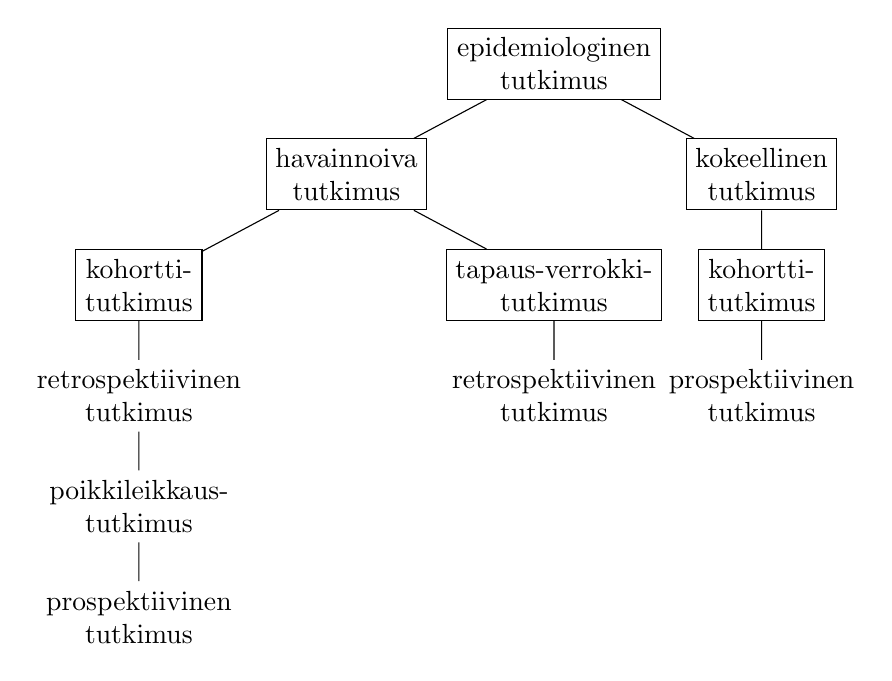
\begin{tikzpicture}
[sibling distance = 15em, level distance = 4em, every node/.style = {shape = rectangle, draw, align = center}]
\node{epidemiologinen\\tutkimus}
   child{node{havainnoiva\\tutkimus}
        child{node{kohortti-\\tutkimus}
            child{node[draw=none,fill=none]{retrospektiivinen\\tutkimus}
                child{node[draw=none,fill=none]{poikkileikkaus-\\tutkimus}
                    child{node[draw=none,fill=none]{prospektiivinen\\tutkimus}}}}}
        child{node{tapaus-verrokki-\\tutkimus}
            child{node[draw=none,fill=none]{retrospektiivinen\\tutkimus}}}}
    child{node{kokeellinen\\tutkimus}
        child{node{kohortti-\\tutkimus}
            child{node[draw=none,fill=none]{prospektiivinen\\tutkimus}}}};
\end{tikzpicture}
\caption{Epidemiologiset tutkimusasetelmat, \cite{twisk13}}
\label{fig:epikaavio}
\end{figure}

\subsection{Pitkittäisaineiston analyysi}

Kuten sanottu, pitkittäisaineistoille on ominaista yhden tai useamman yksilön seuranta usean havaintokerran ajan. Käytännössä useinkaan kaikilta yksilöiltä ei kyetä saamaan samaa määrää havaintoja ja havaintoajankohdat voivat vaihdella. Tällöin puhutaan epätasapainoisesta (\textit{unbalanced}) pitkittäisaineistosta \cite{laird82}.

Mm. \cite{verbeke00, goldstein11} mukaan epätasapainoisen pitkittäisaineiston analyysissa ei suoraan voida hyödyntää yleistä monimuuttujamenetelmien kehikkoa, vaan malli tulee jakaa kahdelle tai useammalle tasolle. 

Samoilta yksilöiltä kerättyjen toistettujen mittausten muodostamassa pitkittäisaineistossa yksilökohtaiset mittausvektorit muodostavat hierarkian ensimmäisen tason ja itse yksilöt toisen tason \cite{goldstein11}.

%Ensimmäisellä tasolla yksilökohtaisten toistomittaussarjojen vektorit tiivistetään pienempään [EPÄMÄÄRÄINEN KÄÄNNÖS] määräänhttps://www.overleaf.com/project/5d7b3ded96d15900017b8b7e yksilökohtaisia regressiokertoimia ja toisella tasolla estimaatit liitetään tunnettuihin taustamuuttujiin hyödyntäen monimuuttujamenetelmiä.

Lineaaristen sekamallien kirjallisuudessa kaksitasoisen lähestymistavan perusteoksena viitataan \cite{laird82} artikkeliin \textit{Random-Effects Models for Longitudinal Data}. Tosin \cite{laird82} esittävät tasot yhtenä lineaarikombinaationa ja vasta myöhemmässä kirjallisuudessa mm. \cite{verbeke00, talbott06} on katsottu luontevaksi esitellä ensin kaksitasoinen malli ja johtaa siitä \cite{laird82} yleinen lineaarisen sekamallin muoto.

Palaamme kaksitasoisen mallin ja yleisen lineaarisen sekamallin määritelmään myöhemmin. [ks LSM]. \\

\subsection{Finlapset aineisto}

Tutkielmassa hyödynnetty aineisto perustuu Terveyden ja hyvinvoinninlaitoksen (THL) Finlapset-rekisterihankkeen (FINLAPSET) ohessa kerättyihin tietoihin lasten ja nuorten  perustuvat lastenneuvoloiden kouluterveydenhuollon ja opiskelijaterveydenhuollon terveydenhoitokäynneillä suoritetuista paino- ja pituusmittauksista. Tiedot on kerätty osana perusterveydenhuollon avohoidon hoitoilmoitusrekisterin (Avohilmo) tietokeräystä.\\

Terveystarkastuksissa kerättävistä tiedoista pituus- ja painotiedot ovat olleet osa Avohilmon tietosisältöä vuodesta 2010 lähtien, mutta tietopuutteiden vuoksi tässä tutkielmassa on mukana tietoja vuodesta 2013 alkaen. \\

Finlapset-rekisterihankkeen keskeisiä tutkimuskysymyksiä olivat lasten ja nuorten ylipaino ja lihavuus sekä pituus- ja painotietojen valtakunnallinen kattavuus. Tarkastelemme seuraavaksi aineiston keskeisiä rajauksia ja teknisiä määrityksiä. \\

\subsubsection{Finlapset-aineiston muodostus}

Avohilmosta suoritetun poiminnan yhteydessä aineistoon on tehty seuraavat rajaukset:

\begin{itemize}
    \item Käynti on tehty vastaanotolla
    \item Käynti on luonteeltaan terveydenhoitokäynti
    \item Käynti on luokiteltu lastenneuvola-, kouluterveydenhuolto-, opiskelijaterveydenhuoltokäynniksi
    \item Lapsen tai nuoren ikä mittaushetkellä on välillä $[1,75;20)$
\end{itemize}

Rajauksillä on pyritty poistamaan mahdollisia harhan lähteitä. Esimerkiksi rajaamalla tarkastelu vain terveydenhoitokäynteihin voidaan sulkea pois sellaisia käyntejä, jotka liittyvät jonkin sairauden hoitoon tai seurantaan. Näillä lapsilla käyntejä voi olla huomattavasti enemmän kuin vertaisillaan ja joihinkin sairauksiin voi myös liittyä epätavallisia painon muutoksia. \\

Paino- ja pituustietojen kirjaaminen tapahtuu sähköisesti potilastietojärjestelmiin, joista ne siirretään osaksi Avohilmoa. Kirjaamiskäytännöt vaihtelevat potilastietojärjestelmittäin ja pituus- ja painomittaukset voivat olla kirjattu eri yksiköissä sekä niissä voi olla inhimillisestä kirjausvirheitä.\\

Edellämainittuja on pyritty karsimaan seuraavilla yksinkertaisilla skaalaussäännöillä:

\begin{itemize}
    \item Paino yli 1000 $\longrightarrow$ yksikkönä g?  $\longrightarrow$ jaetaan 1000:lla kunnes alle 1000
    \item Pituus on yli 300 $\longrightarrow$ yksikkönä mm? $\longrightarrow$ jaetaan 10:llä kunnes alle 300
    \item Pituus pienempää kuin 2,3 $\longrightarrow$ yksikkönä m? $\longrightarrow$ kerrotaan 100
\end{itemize}

Aineistosta rajattiin pois myös biologisesti mahdottomiksi tulkitut mittaukset. Tämä suoritettiin laskemalla painosta ($w$) ja pituudesta ($h$) ensin niiden keskinäistä suhdetta kuvaava painoindeksi (\textit{Body Mass Index, BMI}) tavanomaisella kansainvälisesti vakiintuneella menetelmällä

$$
\textbf{BMI} = \frac{w_{kg}}{h_{m}^2}.
$$

Lapsen ruumiinrakenne, ja siten painon ja pituuden suhde, vaihtelee huomattavasti iän mukaan, joten lapsen iän mukaisen painoindeksin jakauman ääriarvoja voidaan arvioida Colen LMS-menetelmällä \cite{cole90}. LMS-menetelmä, joskus myös \textit{BMI z-score function}, tarjoaa potenssimuunnoksella normalisoidun ja standardisoidun keskihajontapistemäärän, perustuen lapsen kuukausi-iän ja sukupuolen perusteella muodostettuihin parametreihin. Pistemäärä määritellään

$$
\text{BMI}_z = \frac{\bigg( \big( \frac{\text{BMI}}{\mu}\big)^\lambda - 1 \bigg)}{\lambda \ \sigma},
$$

jossa $\lambda$ on jakaumaa normalisoivan potenssimuunnoksen (\textit{Box Cox}) parametri, $\mu$ BMI jakauman odotusarvo ja $\sigma$ jakauman variaatiokerroin. Taulukoidut parametrit ovat saatavilla esimerkiksi Maailman terveysjärjestö WHO:lta ja Yhdysvaltain tautikeskus CDC:ltä.\\

Esimerkiksi 11-vuotiaan pojan taulukoiduilla parametreilla, $\lambda = -1,7862$, $\mu = 16,9392$ ja $\sigma = 0,11070$, painoindeksiä 34 $\frac{kg}{m^2}$ vastaava $\text{BMI}_z$ olisi

$$
\frac{\bigg( \big( \frac{34}{16,9392}\big)^{-1,7862} - 1 \bigg)}{16,9392 \cdot 0,11070} \approx 3,6,
$$

mutta vaikkapa kirjauksessa tapahtuneen näppäilyvirheen takia kirjattu painoindeksi 43 tuottaisi pistemääräksi noin 4,1.\\

Finlapset -hankkeessa kriittiseksi rajaksi valittiin $|\text{BMI}_z| = 4$ ja sitä poikkeavammat mittaukset rajattiin poiminnan ulkopuolelle.\\

LMS-menetelmää on kritisoitu, kuten yllä havaittiin, mm. siitä, että se kuvaa leveän painoindeksiarvojoukon hyvin kapealle välille. Lisäksi vanhemmilla lapsilla äärimmäisenkin korkeat painoindeksiarvot kuvautuvat hyvin lähelle hyväksyttäviksi katsottuja painoindeksin arvoja \cite{flegal13, cdc13}. \\

\cite{flegal13} suosittelevat käyttämään modifioitua pistemäärää, jossa etäisyys jakauman odotusarvosta kuvataan takaisin painoindeksiavaruuteen. Tätä on syytä punnita kehitystarpeena myös Finlapset-hankkeen tulevissa lasten ja nuorten pituus- ja painotietoja käsittelevissä julkaisuissa. \\

Finlapset-hankkeessa havaintoja rajattiin lisäksi siten, että lapsilta ja nuorilta valittiin kunkin tutkimuksessa mukana olleen kalenterivuoden syntymäpäivää lähinnä ollut mittaus. Mikäli yhtäkään mittausta ei ollut 180 vuorokauden absoluuttisella etäisyydellä kalenterivuoden syntymäpäivästä, ei kyseiselle lapselle otettu mittausta mukaan kyseiseltä kalenterivuodelta. \\

Tulokset julkaistiin vuosilta 2014\textendash2018 sellaisilta lapsilta ja nuorilta, jotka olivat mittaushetkellä 2\textendash16-vuotiaita. \\

Tässä tutkielmassa noudatetaan Finlapset-aineiston rajauksia muilta osin, lukuunottamatta rajausta yhteen mittaukseen kalenterivuotta kohden tai julkaisun yhdeydessä suoritettua kalenterivuoden ja iän perusteella tehtyä rajausta. Tutustumme aineistoon seuraavaksi yksinomaan tämän tutkielman piirissä.\\

\subsubsection{Rekisteripohjainen lasten ja nuorten neuvola-ja kouluterveysaineisto pitkittäisaineistona}

Esittäessämme FinLapset aineiston formaalisti pitkittäisaineiston muodossa, voimme, \cite{fitzmaurice11} esitystapaa mukaillen, aloittaa määrittelemällä painoindeksin satunnaismuuttujana $Y_{ij}$ ja aineistosta havaitun arvon $y_{ij}$, jossa $i = 1, \dots, N$ on yksilöön viittaava indeksi ja $j = 1, \dots n_i$ yksilön $i$ mittaukseen viittava indeksi. On tärkeää huomioida, että Finlapset aineistossa lasten mittausmäärät vaihtelevat yksilöittäin, eli on mahdollista, että $n_i \neq n_k$, kun $i,k = 1,\dots, N$ ja $i \neq k$. Finlapset aineisto on siten epätasapainoinen pitkittäisaineisto.\\

Yksilön $i$ painoindeksejä vastaavan satunnaismuuttujan vektori voidaan kirjoittaa $n_i \times 1$ matriisina

$$
\bm{Y}_i = 
\begin{bmatrix}
Y_{i1} \\
Y_{i2} \\
\vdots \\
Y_{in_i} \\
\end{bmatrix}
$$

Mittausajankohta Finlapset aineistossa on käynnin päivämäärä, jolla pituus- ja painomittaus on tehty. Tästä seuraa, että yksilöitä ei ole välttämättä mitattu samoin ajankohtina. Siten eräs ehdokas mittausajankohdaksi on yksilön $i$ $j$:nnen mittauksen päivämäärä $t_{\text{PVM}_{ij}}$.\\

Pitkittäisaineiston aikaskaala voidaan määritellä muillakin tavoin, esimerkiksi lapsen mittausajankohdan desimaali-iän mukaan, jolloin $t_{\text{IKÄ}_{ij}} = \frac{t_{\text{PVM}_{ij}} - t_{\text{SPVM}_{i}}}{365,25}$, jossa $t_{\text{SPVM}_{i}}$ on yksilön $i$ syntymäpäivä. Jakajana käytetään lukua 365,25, jolla pyritään huomioimaan karkausvuoden vaikutus.\\ 

Mittauksiin voi liittyä myös taustatietoja, jotka voivat olla aika-invariantteja (\textit{time invariant}), kuten biologinen syntymäsukupuoli ja -kunta tai ajassa muuttuvia (\textit{time variant}), kuten aika ensimmäisestä mittauksesta tai mittaushetken asuinkunta.\\

Vasteeseen $Y_{ij}$ liittyvät taustatiedot voidaan kirjoittaa $p \times 1$ taustamuuttujavektorina. \\

$$
\bm{X}_{ij} = 
\begin{bmatrix}
X_{ij_{1}} \\
X_{ij_{2}} \\
\vdots \\
X_{ij_{p}} \\
\end{bmatrix},
$$

jossa $i = 1, \dots, N$ ja $j = 1, \dots n_i$. \\ 

Yksilön $i$ taustamuuttujavektorit voidaan kirjoittaa siistimmin matriisina

$$
\bm{X}_{i} = 
\begin{bmatrix}
X_{i_{1}}^\top \\
X_{i_{2}}^\top  \\
\vdots \\
X_{i_{n_i}}^\top  \\
\end{bmatrix}
=
\begin{bmatrix}
X_{i_{11}} & X_{i_{11}} & \dots & X_{i_{1p}} \\
X_{i_{21}} & X_{i_{22}} & \dots & X_{i_{1p}} \\
\vdots & \vdots & \ddots & \vdots \\
X_{i_{n_i1}} & X_{i_{n_i2}} & \dots & X_{i_{n_ip}} \\
\end{bmatrix}
$$\\

Tarkastelemme seuraavaksi FinLapset-aineistoa tämän tutkielman kehikossa.\\

\subsubsection{FinLapset-aineiston kuvaileva tarkastelu}

Alkuperäinen FinLapset-aineisto käsittää painoindeksihavaintoja aikaväliltä 2.1.2013\textendash9.4.2020. Alkuperäisen aineiston tunnuslukuja on selvyyden vuoksi merkitty tähdellä (*). \\

Havaintoja on kaikkiaan $N* = 718080$ yksilöltä ja mittausten kokonaismäärä $n* = \sum\limits_{i = 1}^{N*} n_{i} = 2768012$. \\

Yksilökohtaisissa mittausten määrissä $n_{i}$ on merkittävää vaihtelua. Mittausten yksilökohtaisten määrien mediaani on 4, kvartiiliväli $[2,5]$ ja vaihteluväli $[1,116]$.

\begin{table}[ht]
\centering
\begin{tabular}{lrr}
\toprule
$n_i$ & N* & N\\
\midrule
1 & 136319 & 23614\\
2 & 103017 & 20169\\
3 & 103836 & 21116\\
4 & 107896 & 20187\\
5 & 100783 & 17071\\
\addlinespace
6 & 79459 & 12145\\
7 & 46876 & 6587\\
8 & 21040 & 2811\\
9 & 8420 & 1160\\
10 & 3981 & 486\\
\addlinespace
11 & 2174 & 263\\
12 & 1246 & 114\\
13 & 805 & 84\\
14 & 528 & 40\\
15 & 376 & 35\\
\addlinespace
16 & 289 & 28\\
17 & 197 & 9\\
18 & 171 & 7\\
19-29 & 566 & 23\\
30- & 101 & 4\\
\bottomrule
\end{tabular}
\caption{Mittausmäärien jakauma}
\end{table}


\section{Lineaarinen sekamalli}

Lineaariset sekamallit (LSM) ovat tilastollisten mallien joukko lähtökohtaisesti [?] jatkuville vastemuuttujille, joiden jäännösvirheet (residuaalit) ovat normaalisti jakautuneita, mutta eivät välttämättä riippumattomia tai niiden varianssi ei ole vakio \cite{west14}. Kyseisten mallien joukkoa kuvaava, yleisesti käytössä oleva englanninkielinen nimi \textit{linear mixed (effect) model}, juontuu mallien ominaisuuksista siten, että mallit ovat parametreiltään lineaarisia ja niihin voi liittyä taustamuuttujien muodossa sekä \textit{kiinteitä} (\textit{fixed}) ja \textit{satunnaisia} (\textit{random}) vaikutuksia (\textit{effects}) \cite{west14}.

\cite{laird82} kuvaavat kiinteiden ja satunnaisvaikutusten yhteyttä seuraavalla tavalla: Olkoon toistettujen mittausten yksilökohtaiset todennäköisyysjakaumat samaa muotoa (\textit{form}) kaikille yksilöille [ENSIMMÄINEN TASO, KIINT. VAIK.], mutta sallittakoon näiden todennäköisyysjakaumien parametrien vaihtelu yksilöiden välillä. Näiden populaation \textit{satunnaisvaikutusten} parametrien jakauma muodostaa mallin toisen tason [TOINEN TASO, SAT. VAIK.].

Siirtääksemme \cite{laird82} esittämän esimerkin FinLapset-aineiston kehikoon oletamme siis, että yksittäisen lapsen painoindeksin ja valittujen taustamuuttujien (esimerkiksi ikä, sukupuoli jne.) välinen yhteys on lineaarinen, mutta kutakin lasta kohden sovitetun lineaarisen regression parametrit voivat vaihdella. Siten, ehdollisesti yksittäisen lapsen parametrejä kohtaan ja, että populaation regressioparametrit noudattavat 2-ulotteista normaalijakaumaa, toistettujen mittausten reunajakauma noudattaa moniulotteista normaalijakaumaa asetelmaa vastaavalla kovarianssirakenteella. 

EHKÄ YKSINKERTAISTUS? JA LISÄÄ: They (LMMs) allow explicit modelling and analysis of between- and within individual variation.

\subsection{Lineaarisen sekamallin määritelmä}

Jotta voimme perusteellisesti ymmärtää lineaarisen sekamallin luonteen, aloitamme tarkastelun hyvin yleisestä tilastollisen mallin esitysmuodosta, yksinkertaisesta lineaarisesta regressiomallista mallista.

\subsubsection{Lineaarinen regressio}

Olkoon $y_i$ satunnaismuuttujan $Y_i$ havaittu arvo, $x_i$ satunnaismuuttujan $X_i$ havaittu arvo, $\beta_0$ (vakiotermi) ja $\beta_1$ (taustamuuttujan $x_i$ regressiokerroin) kiinteät, mutta tuntemattomat regressiokertoimet ja satunnaismuuttuja $\epsilon_i$ mallin selittämätön osa (jäännöstermi) havainnoille $i = 1,\dots,n$.

Satunnaismuuttujan $Y_i$ ja taustamuuttujan $x_i$ yhteyttä kuvaa yksinkertainen lineaarinen regressiomalli

$$
Y_i = \beta_0 + \beta_1 x_i + \epsilon_i
$$

Laajennettuna useaan usean taustamuuttujan lineaariseen regressioon edellinen voidaan esittää muodossa

$$
Y_i = \beta_0 + \beta_1 x_{i1} + \dots + \beta_p x_{ip} + \epsilon_i
$$

Tiivistääksemme edellistä muotoa, voimme määritellä sarakevektorit $\bm{x_i} = [x_i1 , \dots, x_{ip}]^\top$ ja $\bm{\beta} = [\beta_1 , \dots, \beta_{p}]^\top$ ja kirjoittaa mallin muodossa

$$
Y_i = \bm{x_i}^\top \bm{\beta} + \epsilon_i
$$

havainnoille $i = 1,\dots,n$. \\

%[TARPEETON?] Lopuksi voimme tiivistää mallia edelleen määritellen kullekkin mallin termille havaintokohtaiset vektorit

%$$
%\begin{aligned}
%\begin{bmatrix} 
%Y_1 \\
%\vdots \\
%Y_n \\
%\end{bmatrix}&=
%\begin{bmatrix} 
%\bm{x}_1^\top \\
%\vdots \\
%\bm{x}_n^\top \\
%\end{bmatrix}
%\begin{bmatrix} 
%\beta_1 \\
%\vdots \\
%\beta_p \\
%\end{bmatrix}&&+
%\begin{bmatrix} 
%\epsilon_1 \\
%\vdots \\
%\epsilon_n \\
%\end{bmatrix} \\
%\bm{Y}\quad&=\quad \bm{X}\bm{\beta}&&+\quad \bm{\epsilon}
%\end{aligned}
%$$

[VIELÄ YKSI VÄLIVAIHE? ESIM \cite{fitzmaurice11} s. 76 HISTORICAL APPROACHES; repeated measures anova]


Seuraavaksi hyödynnämme lineaarisen mallin määritelmää esitellessämme lineaariselle sekamallille ensin kaksitasoisen mallin, jonka jälkeen etenemme luontevasti tasot yhdistävään \cite{laird82} yleiseen lineaariseen sekamalliin.

\subsubsection{Kaksitasomalli}

Monitasomalleille keskeistä on aineiston hierarkkisen rakenteen huomioiminen mallissa \textit{satunnaisvaikutusten} avulla \cite{talbott06}. Pitkittäisaineistoa kuvaavassa kaksitasomallissa hierarkian ensimmäinen taso käsittää yksilön mittauskertojen välisen vaihtelun ja toinen taso yksilöiden välisen vaihtelun. Monitasomallit voidaan yleistää myös useammalle tasolle \cite{goldstein11, burzykowski13}.

\paragraph{Ensimmäinen taso}\mbox{}\\

Ensimmäisellä tasolla oletamme kunkin yksilön keskimääräisen vasteen (\textit{Mean response}) noudattavan lineaarista regressiomallia samoilla taustamuuttujilla, mutta yksilöllisillä regressiokertoimilla \cite{fitzmaurice11}. 

Edellistä mukaillen, voimme esittää ensimmäisen tason muodossa

$$
\bm{Y}_i = \bm{Z}_i \bm{\beta}_i + \bm{\epsilon}_i,
$$

jossa $\bm{Y}_i$ on yksilön $i$ $n_i$-vastevektori, $\bm{\beta}_i$ tuntemattomat regressiokertoimet sisältävä $q$-vektori ja $\bm{Z}_i \bm{\beta}_i$ yksilön $i$ tuntematon keskimääräinen vasteen kehitys (\textit{Response trajectory}). Ensimmäisen tason kontekstissa matriisi $\bm{Z}_i$ määrittelee kuinka yksilön keskimääräinen vaste muuttuu ajassa, mutta määritelmä tulee vaatimaan tarkennusta.

Niin sanottujen yksilöiden välillä vaihtelevien kiinteiden, mutta tuntemattomien vaikutusten lisäksi ensimmäiseen tasoon liittyy myös yksilön $i$ mittauksia koskeva satunnaisvirhe $\bm{\epsilon_i}$, jossa $\bm{\epsilon_i} \sim N(0,\bm{R}_i)$, jossa $\bm{R}_i$ on jokin $n_i \times n_i$ kovarianssimatriisi. Yksinkertaisuuden vuoksi voimme olettaa, että $\bm{R}_i = \sigma^2\bm{I}_{n_i}$

Kuvataksemme täsmällisemmin mallin osia, voimme esittää mallin yksilön $i$ vastelle aukikirjoitettussa matriisimuodossa

$$
\begin{bmatrix}
Y_{i1} \\
\vdots \\
Y_{in_{i}} \\
\end{bmatrix}=
\begin{bmatrix}
1 & t_{i1} \\
\vdots \\
1 & t_{in_{i}} \\
\end{bmatrix}+
\begin{bmatrix}
\beta_{1i} \\
\beta_{2i} \\
\end{bmatrix}+
\begin{bmatrix}
e_{i1} \\
\vdots \\
e_{in_{i}} \\
\end{bmatrix}
$$

\paragraph{Toinen taso}\mbox{}\\

Toisella tasolla tuomme malliin oletuksen, että yksilökohtaiset vaikutukset $\bm{\beta}_i$ ovat satunnaismuuttujia jollakin odotusarvolla ja kovarianssilla.

Keskeistä on $\bm{\beta}_i$ yksilöiden välisen vaihtelun mallintaminen mittausajankohdasta riippumattomien vasteen yksilöllisiä eroja selittävinen taustamuuttujien funktiona \cite{fitzmaurice11}.

Siten $\bm{\beta}_i$ odotusarvoksi saamme

$$
\text{E}(\bm{\beta}_i) = \bm{K}_i \bm{\beta},
$$

jossa $\bm{K}_i$ on yksilöiden välistä vaihtelua selittävien muuttujien $(q \times p)$ matriisi.

Yksilöiden välistä residuaalivaihtelua, jota $\bm{K}_i$ ei selitä, merkitsemme

$$
\text{Cov}(\bm{\beta}_i) = \bm{G}.
$$

Lopuksi voimme yhdistää ensimmäisen ja toisen tason komponentit esittääksemme $\bm{Y}_i$:lle lineerisen sekamallin yleisen muodon \cite{fitzmaurice11, verbeke00}.

\subsubsection{Yleinen lineaarinen sekamalli}

Yhdistääksemme ensimmäisen ja toisen tason, hyödyntäen toisen vaiheen oletuksia, voimme kirjoittaa $\bm{\beta}_i$ uudelleen muodossa

$$
\bm{\beta}_i = \bm{K}_i \bm{\beta} + \bm{b}_i,
$$

jossa $\bm{b}_i \sim N(0,\bm{G})$ \\

Tässä $\bm{b}_i$ kuvaa $i$:nnen yksilön poikkeamaa keskimääräisestä vasteesta, kun yksilöiden yhteiset taustamuuttujat on huomioitu \cite{fitzmaurice11}.

Yhdistetty muoto saadaan sijoittamalla

$$
\begin{aligned}
\bm{Y}_i &= \bm{Z}_i \bm{\beta_i} + \bm{\epsilon}_i \\
&= \bm{Z}_i (\bm{K}_i \bm{\beta} + \bm{b}_i) + \bm{\epsilon}_i \\
&= (\bm{Z}_i \bm{K}_i) \bm{\beta} + \bm{Z}_i \bm{b}_i + \bm{\epsilon}_i \\
&= \bm{X}_i \bm{\beta} + \bm{Z}_i \bm{b}_i + \bm{\epsilon}_i, \\
\end{aligned}
$$

jossa $\bm{X}_i = \bm{Z}_i \bm{K}_i$. \\

Yleisesti muotoiltuna, malli joka tyydyttää vaatimukset

$$
\left\{
    \begin{array}{ll}
        \bm{Y}_i = \bm{X}_i \bm{\beta} + \bm{Z}_i \bm{b}_i + \bm{\epsilon}_i \\
        \bm{b}_i \sim N(0,\bm{G}) \\
        \bm{\epsilon}_i \sim N(0,\bm{R}_i) \\
        \bm{b}_i, \dots , \bm{b}_N \perp \bm{\epsilon}_i, \dots , \bm{\epsilon}_N 
    \end{array}
\right.
$$

on lineaarinen sekamalli \cite{verbeke00, laird82}.\\


\cite{fitzmaurice11} alleviivaavat, että kaksitasomalliin, sen ollessa pedagogisesti hyödyllinen lineaarisen sekamallin yksilöiden välisten ja yksilökohtaisten vaikutusten esitystapa, liittyy merkittävä rajoite, sillä muoto  $\bm{X}_i = \bm{Z}_i \bm{K}_i$ edellyttää, että $\bm{K}_i$ sisältää vain yksilöiden välisiä vaikutuksia selittäviä muuttujia ja $\bm{Z}_i$ vain yksilökohtaisia ajassa muuttuvia vaikutuksia selittäviä muuttujia.

Tämä rajoite on kuitenkin kierrettävissä olettamalla, että $\bm{X}_i$ on lineaarisen sekamallin mielivaltainen koematriisi ja, että $\bm{Z}_i$ muodostuu sarakkeista, jotka ovat $\bm{X}_i$ sarakkeiden osajoukko. Tällöin vasteen $\bm{Y}_i$ odotusarvo yli kaikkien yksilökohtaisten vaikutusten

$$
\text{E}(\bm{Y}_i) = \bm{X}_i \bm{\beta}, \\
$$

määrittelee vasteen keskimääräisen kehityksen koko tarkasteltavana olevalle joukolle ja $\bm{Z}_i \bm{b}_i$ kuvaa selittämättä jäänyttä osaa, eli yksilökohtaisia poikkeamia tarkastelujoukon vasteen keskimääräisestä kehityksestä \cite{fitzmaurice11}. \\

Täsmällisemmin muotoiltuna, tarkastellaan ehdollista odotusarvoa

$$
\text{E}(\bm{Y}_i | \bm{b}_i) = \bm{X}_i \bm{\beta} + \bm{Z}_i \bm{b}_i.
$$

Koska $\text{E}(\bm{b}_i) = 0$, saamme reunajakauman $\bm{Y}_i$ odotusarvoksi

$$
\begin{aligned}
\text{E}(\bm{Y}_i) &=  \text{E}(\text{E}(\bm{Y}_i | \bm{b}_i)) \\
&=  \text{E}(\bm{X}_i \bm{\beta} + \bm{Z}_i \bm{b}_i) \\
&=  \bm{X}_i \bm{\beta} + \bm{Z}_i \text{E}(\bm{b}_i) \\
&=  \bm{X}_i \bm{\beta}. \\
\end{aligned}
$$

Siten vahvistamme tulkinnan, että parametrit $\bm{\beta}$ kuvaavat koko tarkastelujoukon yhteisiä, niin kutsuttuja \textit{kiinteitä} vaikutuksia ja ottaen huomioon kiinteät vaikutukset, $\bm{b}_i$ kuvaa yksilön $i$ poikkeamaa koko tarkastelujoukon keskimääräisesta vasteesta, toisin sanoen mallin \textit{satunnaisvaikutuksia}. \\

\cite{fitzmaurice11} mukaan lineaarisen sekamallin kaksitasoesitys asettaa erityisvaatimuksia myös mallin kovarianssille. Koska kovarianssirakenteella on monin tavoin keskeinen asema, sekä yleisen lineaarisen sekamallin teoriassa, että pitkittäisaineiston erityistapauksessa, erotamme sen käsittelyn omaksi osiokseen.\\ 

\subsection{Kovarianssirakenteet}

Tarkastellaan seuraavaksi lineaarisen sekamallin kovarianssirakenteita \cite{fitzmaurice11} esittämässä yleisessä muodossa. Lähtökohtana on erottaa yksilökohtaisen ja yksilöiden välisen vaihtelun lähteet ja mahdollistaa näiden yksikäsitteinen analyysi.\\

Yleisen lineaarisen sekamallin

$$
\bm{Y}_i = \bm{X}_i \bm{\beta} + \bm{Z}_i \bm{b}_i + \bm{\epsilon}_i \\
$$

tapauksessa voimme, edellisessä luvussa esitetyn määritelmän mukaan, esittää yksilön $i$ keskimääräisen vasteen ehdollisena odotusarvona

$$
\text{E}(\bm{Y}_i | \bm{b}_i) = \bm{X}_i \bm{\beta} + \bm{Z}_i \bm{b}_i, \\
$$

jossa otamme huomioon yksilön $i$ poikkeaman $\bm{b}_i$ koko tutkimusjoukon keskimääräisestä vasteesta.

Pyrkimyksessämme erottaa yksilön $i$ mittausten keskinäinen vaihtelu koko tutkimusjoukon mittausten vaihtelusta, määritellään yksilön $i$ mittausten kovarianssi samaan tapaan ehdollisena kovarianssina 

$$
\text{Cov}(\bm{Y}_i | \bm{b}_i) = \text{Cov}(\bm{\epsilon}_i) = \bm{R}_i,
$$

jolloin \cite{fitzmaurice11} mukaan reunajakauman $\bm{Y}_i$ kovarianssiksi saamme

$$
\begin{aligned}
\text{Cov}(\bm{Y}_i) &= \text{Cov}(\bm{X}_i \bm{\beta} +\bm{Z}_i\bm{b}_i + \bm{\epsilon}_i) \\
&= \text{Cov}(\bm{Z}_i \bm{b}_i) + \text{Cov}(\bm{\epsilon}_i) \\
&= \bm{Z}_i \text{Cov} (\bm{b}_i) \bm{Z}^\top_i + \text{Cov}(\bm{\epsilon}_i)\\
&= \bm{Z}_i \bm{G} \bm{Z}^\top_i + \bm{R}_i.\\
\end{aligned}
$$ \\

Näin ollen, lineaarinen sekamalli mahdollistaa yksilöiden välisten varianssilähteiden $\bm{G}$ ja yksilökohtaisten varianssilähteiden $\bm{R}_i$ yksikäsitteisen analyysin. \\

Koska mallin kovarianssi esitetään mittausajankohtien funktiona, ei satunnaisvaikutusten kovarianssirakenne vaadi tasapainoista asetelmaa pitkittäisaineistossa, kovarianssiparametrien määrä ei riipu mittausajankohdista tai niiden lukumäärästä ja varianssi sekä kovarianssi voivat myös muuttua mittausajankohtien funktiona, mistä on merkittävää hyötyä epätasapainoisen pitkittäisaineiston analyysissä \cite{fitzmaurice11}. \\

Kirjoitetaan yksilöiden välisten satunnaisvaikutusten $q$-vektori $\bm{b}_i \sim N(0,\bm{G})$ yksilölle $i$ matriisimuodossa

$$
\bm{b}_i =
\begin{bmatrix}
\text{b}_{1i} \\
\vdots \\
\text{b}_{qi} \\
\end{bmatrix},
$$

jolloin kovarianssi  $\text{Cov}(\bm{b}_i) = \bm{G}$ voidaan esittää muodossa

$$
\bm{G} =
\begin{bmatrix}
\text{Var}(\text{b}_{1i}) & \dots & \text{Cov}(\text{b}_{1i}, \text{b}_{qi}) \\
\vdots & \ddots & \vdots \\
\text{Cov}(\text{b}_{1i}, \text{b}_{qi}) & \dots & \text{Var}(\text{b}_{qi}) \\
\end{bmatrix}. \\
$$

Lisäksi kirjoitetaan yksilön $i$ mittausten $n_i$ satunnaisvirhe, eli residuaali $\bm{\epsilon}_i \sim N(0,\bm{R}_i)$ yksilölle $i$ matriisimuodossa

$$
\bm{\epsilon}_i =
\begin{bmatrix}
\epsilon_{1i} \\
\vdots \\
\epsilon_{n_{i}i} \\
\end{bmatrix},
$$

jolloin kovarianssi  $\text{Cov}(\bm{\epsilon}_i) = \bm{R}_i$ voidaan esittää muodossa

$$
\bm{R}_i =
\begin{bmatrix}
\text{Var}(\epsilon_{1i}) & \dots & \text{Cov}(\epsilon_{1i}, \epsilon_{n_{i}i}) \\
\vdots & \ddots & \vdots \\
\text{Cov}(\epsilon_{1i}, \epsilon_{n_{i}i}) & \dots & \text{Var}(\epsilon_{qi}). \\
\end{bmatrix}
$$

\cite{burzykowski13, west14} mukaan matriisin $\bm{G}$ alkiot voidaan kuvata jonkin kovarianssiparametrivektorin $\bm{\theta}$ alkioiden funktioina $\bm{G} = \sigma(\bm{\theta}_G)$.\\

Jos emme aseta muita vaatimuksia, kuin että $q \times q$ matriisi $\bm{G}$ on symmetrinen ja positiivisesti definiitti käytetään nimitystä \textit{rakenteeton} kovarianssirakenne. Tässä tapauksessa $\bm{G}$ symmetrisyyden johdosta $\bm{\theta}_G$ sisältää $(q(q + 1))/2$ parametria \cite{burzykowski13, west14}.\\

Tarkastellaan tarkemmin matriisin $\bm{G}$ mahdollisia kovarianssirakenteita. Esimerkiksi jos rakenteettoman kovarianssirakenteen tapauksessa oletetamme malliin kaksi satunnaisvaikutusta, satunnaisen vakiotermin ja satunnaisen kulmakertoimen. Tällöin kovarianssiparametrien määrä olisi $q=2(2+1)/2=3$, jolloin $\bm{\theta}_G$ voitaisiin kirjoittaa muodossa\\

$$
\bm{\theta}_G =
\begin{bmatrix}
\sigma^2_{\text{b}_{1i}}\\
\sigma_{\text{b}_{1i}, \text{b}_{2i}} \\
\sigma^2_{\text{b}_{2i}} \\
\end{bmatrix}\\
$$

ja $\bm{G}$ muodossa \\

$$
\begin{aligned}
\bm{G} &=
\begin{bmatrix}
\text{Var}(\text{b}_{1i}) & \text{Cov}(\text{b}_{1i}, \text{b}_{2i}) \\
\text{Cov}(\text{b}_{1i}, \text{b}_{2i}) & \text{Var}(\text{b}_{2i}) \\
\end{bmatrix} \\
&=
\begin{bmatrix}
\sigma^2_{\text{b}_{1i}} & \sigma_{\text{b}_{1i}, \text{b}_{2i}} \\
\sigma_{\text{b}_{1i}, \text{b}_{2i}} & \sigma^2_{\text{b}_{2i}} \\
\end{bmatrix} \\
\end{aligned}
$$

Matriisin $\bm{G}$ rakennetta voidaan yksinkertaistaa vaihtoehtoisilla parametrisoinneilla kuten esimerkiksi \textit{varianssikomponenttirakenteessa}, jossa jokaisella satunnaisvaikutuksella $\bm{b_i}$ on yksilöllinen varianssi ja kovarianssit ovat rajoitettu nollaan. Tässä tapauksessa $\bm{\theta}_G$ \\

$$
\bm{\theta}_G =
\begin{bmatrix}
\sigma^2_{\text{b}_{1i}}\\
\sigma^2_{\text{b}_{2i}} \\
\end{bmatrix}\\
$$

määrittelee matriisin $\bm{G}$ diagonaalin \\

$$
\bm{G} =
\begin{bmatrix}
\sigma^2_{\text{b}_{1i}} & 0 \\
0 & \sigma^2_{\text{b}_{2i}} \\
\end{bmatrix} \\
$$

Rakenteeton kovarianssirakenne ja varianssikomponenttirakenne ovat yleisimmin sovelletut matriisin $\bm{G}$ rakenteet, mutta myös muita rakenteita on esitetty \cite{west14}. \\

Siirrytään tarkastelemaan matriisin $\bm{R}_i$ mahdollisia kovarianssirakenteita. Määritellään samoin $\bm{R}_i$ alkiot kovarianssiparametrivektorin $\bm{\theta_R}$ alkioiden funktioina.\\

Yksinkertaisin kovarianssirakenne matriisille $\bm{R}_i$ on diagonaalirakenne, jossa yksilön $i$ mittauksiin liittyvät residuaalit oletetaan keskenään korreloimattomiksi ja niiden varianssit vakioiksi. Diagonaalimatriisi $\bm{R}_i$ on muotoa\\

$$
\bm{R}_i =
\begin{bmatrix}
\sigma^2 & \dots & 0 \\
\vdots & \ddots & \vdots \\
0 & \dots & \sigma^2 \\
\end{bmatrix}
$$

ja parametrivektori $\bm{\theta}_R = [\sigma^2]$ sisältää vain yhden parametrin. Yksilöiden $i$ mittausten välillä ei siis oleteta olevan korrelaatiota, mikä pitkittäisaineiston tapauksessa on hyvin epärealistinen oletus. \\

Eräänä yksinkertaisena vaihtoehtona on esitetty \textit{tasakorrelaatiorakennetta}, jossa yksilön $i$ mittausten residuaaleille oletetaan vakiokorrelaatio. \\

$$
\bm{R}_i =
\begin{bmatrix}
\sigma^2 + \sigma_1 & \dots & \sigma_1 \\
\vdots & \ddots & \vdots \\
\sigma_1 & \dots & \sigma^2 + \sigma_1 \\
\end{bmatrix}
$$

jonka parametrit muodostavat parametrivektorin

$$
\bm{\theta}_R =
\begin{bmatrix}
\sigma^2\\
\sigma_1 \\
\end{bmatrix}\\
$$

Vaikka tasakorrelaatiorakenteen esitetään soveltuvan tilanteisiin, joissa toistetut mittaukset suoritetaan identtisissä olosuhteissa \cite{pinheiro00, west14}, sitä pidetään yleisesti liian optimistisena pitkittäisaineiston kannalta \cite{pinheiro00, fitzmaurice11, west14}.\\

On luontevaa ajatella pitkittäisaineiston yksilön $i$ mittausten välillä vallitsevan jokin korrelaatio ja ajallisesti lähellä olevien mittaukset olevan samankaltaisempia kuin ajallisesti etäämmällä olevien. Yksilön mittausten residuaaleja kuvaavan kovarianssirakenteen tulisi siis heijastaa tällaista asetelmaa.\\

Tasapainoisen pitkittäisaineiston tapauksessa \textit{autoregressiivinen} kovarianssirakenne on usein sopiva valinta.

$$
\bm{R}_i =
\begin{bmatrix}
\sigma^2 & \sigma^2 \rho & \dots  & \sigma^2 \rho^{n_i -1} \\
\sigma^2 \rho   & \sigma^2      & \dots & \sigma^2 \rho^{n_i -2} \\
\vdots   & \vdots        & \ddots & \vdots \\
\sigma^2 \rho^{n_i -1} & \sigma^2 \rho^{n_i -2} & \dots & \sigma^2 \\
\end{bmatrix}
$$

parametrivektorilla \\

$$
\bm{\theta}_R =
\begin{bmatrix}
\sigma^2\\
\rho \\
\end{bmatrix}\\
$$

Käytännön tapauksissa, koskien vaikkapa epätasapainoista pitkittäisaineistoa, on usein tarve joustavammalle matriisin $\bm{R}_i$ kovarianssirakenteelle. Sopivan rakenteen valinta vaatii kuitenkin havaitun aineiston ja tutkittavan ilmiön ominaisuuksien tarkastelua. Tähän prosessiin palaamme myöhemmin tutkielmassa.\\

\subsection{Estimointi}

Estimoinnin näkökulmasta kiinnostuksen kohteena ovat kiinteiden vaikutusten parametrit $\bm{\beta}$ ja kovarianssiparametrit $\bm{\theta}_G$ ja $\bm{\theta}_R$. Yleisimmät menetelmät edellä mainittujen parametrien estimointiin ovat suurimman uskottavuuden (\textit{maximum likelihood, ML}) ja rajoitettu suurimman uskottavuuden (\textit{restricted maximum likelihood, REML}) menetelmät \cite{west14}. \\

Suurimman uskottavuuden menetelmässä tavoitteena on uskottavuusfunktion maksimointi. Uskottavuusfunktio on mallin parametrien funktio ja sen globaali maksimi, parametrin suurimman uskottavuuden estimaatti, on parametrin arvo jolla havaittu aineisto on uskottavin \cite{casella02}. \\

Lineaarisen sekamallin tapauksessa uskottavuuspäättely perustuu parametrivektoreista $\bm{\beta}$ ja $\bm{\theta} = [\bm{\theta}_G, \bm{\theta}_R]^\top$ ja $\bm{Y}_i$ reunajakaumasta muodostettuun uskottavuusfunktioon. \\

Reunajakauman uskottavuusfunktion muodostamiseksi mm. \cite{west14} ehdottavat lineaarisen sekamallin yleiseen muotoon läheisesti liittyvää marginaalimallia. \cite{west14} mukaan lineaarisen sekamallin yleisestä muodosta voidaan päätellä (\textit{imply}) seuraava marginaalimalli \\

$$
\bm{Y}_i = \bm{X}_i \bm{\beta} + \bm{\epsilon}_i, \\
$$

jossa

$$
\bm{\epsilon}_i \sim N(0,\bm{V}_i) \\
$$

ja kovarianssimatriisi $\bm{V}_i$ määritellään\\

$$
\bm{V}_i = \bm{Z}_i \bm{G} \bm{Z}^\top_i + \bm{R}_i \\
$$

\cite{west14} painottavat, että marginaalimalli ei ole ekvivalentti lineaarisen sekamallin yleisen muodon kanssa, sillä marginaalimalli ei sisällä satunnaisvaikutuksia. Satunnaisvaikutuksia vastaava kovarianssirakenne on kuitenkin mahdollista sisällyttää malliin matriisin $\bm{V}_i$ kautta.\\

Päättellyn marginaalimallin avulla voimme määritellä vasteen $\bm{Y}_i$ reunajakauman moniulotteisena normaalijakaumana \\

$$
\bm{Y}_i \sim N(\bm{X}_i \bm{\beta}, \bm{Z}_i \bm{G} \bm{Z}^\top_i + \bm{R}_i)
$$

Huomioitavaa on, että $\bm{Z}_i \bm{G} \bm{Z}^\top_i$ kuvastaa yksilöiden välistä vaihtelua ja $\bm{R}_i$ yksilön $i$ mittausten sisäistä vaihtelua. \\

Koska $\bm{V}_i = \bm{Z}_i \bm{G} \bm{Z}^\top_i + \bm{R}_i$ on funktio $\bm{V}_i(\bm{\theta})$ kovarianssiparametreillä $\bm{\theta}$, voimme määritellä marginaalimallia vastaavan tiheysfunktion $f(\bm{Y}_i \, | \, \bm{\beta}, \bm{\theta})$ muodossa 

$$
f(\bm{Y}_i;\bm{\beta}, \bm{\theta}) = (2\pi)^{-\frac{n_i}{2}} \det (\bm{V}_i)^{-\frac{1}{2}} \exp \big( -\frac{1}{2} [\bm{Y}_i - \bm{X}_i \bm{\beta}]^\top \bm{V}_i^{-1} [\bm{Y}_i - \bm{X}_i \bm{\beta}]\big),
$$

jolloin havaitun aineiston $\bm{Y}_i = \bm{y}_i$ uskottavuusfunktioksi saamme $m$ riippumattoman kontribuution tulona \\

$$
\begin{aligned}
L(\bm{\beta}, \bm{\theta};\bm{y}) &= \prod_{i=1}^{m} f(\bm{y}_i;\bm{\beta}, \bm{\theta}) \\
&= \prod_{i=1}^{m} (2\pi)^{-\frac{n_i}{2}} \det (\bm{V}_i)^{-\frac{1}{2}} \exp \big( -\frac{1}{2} [\bm{y}_i - \bm{X}_i \bm{\beta}]^\top \bm{V}_i^{-1} [\bm{y}_i - \bm{X}_i \bm{\beta}]\big), \\
\end{aligned}
$$

jossa $i = (1,\dots, m)$. Vastaava log-uskottavuusfunktio saadaan luonnollisella logaritmilla

$$
\begin{aligned}
l(\bm{\beta}, \bm{\theta};\bm{y}) &= \log (\prod_{i=1}^{m} f(\bm{y}_i \, ; \, \bm{\beta}, \bm{\theta})) \\
&= \log \bigg(\prod_{i=1}^{m} (2\pi)^{-\frac{n_i}{2}} \det (\bm{V}_i)^{-\frac{1}{2}} \exp \big( -\frac{1}{2} [\bm{y}_i - \bm{X}_i \bm{\beta}]^\top \bm{V}_i^{-1} [\bm{y}_i - \bm{X}_i \bm{\beta}]\big) \bigg), \\
&= \log \bigg(\prod_{i=1}^{m} (2\pi)^{-\frac{n_i}{2}} \bigg) + \log \bigg(\prod_{i=1}^{m} \det (\bm{V}_i)^{-\frac{1}{2}} \bigg) \\
&\quad + \log \bigg(\prod_{i=1}^{m} \exp \big( -\frac{1}{2} [\bm{y}_i - \bm{X}_i \bm{\beta}]^\top \bm{V}_i^{-1} [\bm{y}_i - \bm{X}_i \bm{\beta}]\big) \bigg) \\
&= -\frac{1}{2} \sum\limits_{i=1}^{m} n_i \log (2\pi) -\frac{1}{2} \sum\limits_{i=1}^{m} \log (\det (\bm{V}_i)) -\frac{1}{2} \sum\limits_{i=1}^{m} [\bm{y}_i - \bm{X}_i \bm{\beta}]^\top \bm{V}_i^{-1} [\bm{y}_i - \bm{X}_i \bm{\beta}] \\
&= -\frac{1}{2} n \log (2\pi) -\frac{1}{2} \sum\limits_{i=1}^{m} \log (\det (\bm{V}_i)) -\frac{1}{2} \sum\limits_{i=1}^{m} [\bm{y}_i - \bm{X}_i \bm{\beta}]^\top \bm{V}_i^{-1} [\bm{y}_i - \bm{X}_i \bm{\beta}], \\
\end{aligned}
$$

jossa $n = \sum\limits_{i=1}^{m} n_i$.\\

\cite{west14} mukaan olisi mahdollista estimoida $\bm{\beta}_i$ ja $\bm{\theta}$ samanaikaisesti, mutta käytännössa algoritminen optimointi suoritetaan usein \textit{profiloimalla} $\bm{\beta}$ ulos log-uskottavuusfunktioista. \\

Vaikka yleisessä tapauksessa $\bm{\theta}$ on tuntematon, sellaisen erityistapauksen käsittely, että $\bm{\theta}$ on tunnettu, tarjoaa tärkeän välivaiheen lopullisen profiili-log-uskottavuusfunktion muodostamiseksi.\\

Parametrivektorin $\bm{\theta}$ ollessa tunnettu, estimoitavaksi jäävät ainoastaan kiinteät vaikutukset $\bm{\beta}_i$. Log-uskottavuusfunktio on tällöin vain parametrin $\bm{\beta}_i$ funktio ja sen optimointion yhteensopivaa tappiofunktion (\textit{loss function}) $q(\bm{\beta})$ minimoinnin kanssa, joka määritellään

$$
q(\bm{\beta}) = \frac{1}{2} \sum\limits_{i=1}^{m} [\bm{y}_i - \bm{X}_i \bm{\beta}]^\top \bm{V}_i^{-1} [\bm{y}_i - \bm{X}_i \bm{\beta}].
$$

Funktion $q(\bm{\beta})$ optimointi voidaan suorittaa yleistetyllä pienimmän neliösumman menetelmällä.

Derivoimalla log-uskottavuusfunktio $\bm{\beta}$ suhteen saamme

$$
\begin{aligned}
\frac{\partial L(\bm{\beta}, \bm{\theta};\bm{y})}{\partial \bm{\beta}} &= \sum\limits_{i=1}^{m}\bm{X}_{i}^\top \bm{V}_i^{-1} (\bm{y}_i - \bm{X}_{i} \bm{\beta})
\end{aligned}
$$

ja asettamalla $\sum\limits_{i=1}^{m}\bm{X}_{i}^\top \bm{V}_i^{-1} (\bm{y}_i - \bm{X}_{i} \bm{\beta}) = 0$ saamme normaaliyhtälömuodon

$$
\begin{aligned}
\sum\limits_{i=1}^{m}\bm{X}_{i}^\top \bm{V}_i^{-1} (\bm{y}_i - \bm{X}_{i} \bm{\beta}) &= 0 \\
\sum\limits_{i=1}^{m}\bm{X}_{i}^\top \bm{V}_i^{-1}\bm{y}_i - \sum\limits_{i=1}^{m}(\bm{X}_{i}^\top \bm{V}_i^{-1}\bm{X}_{i}) \bm{\beta} &= 0 \\
 \sum\limits_{i=1}^{m}(\bm{X}_{i}^\top \bm{V}_i^{-1}\bm{X}_{i}) \bm{\beta} &= \sum\limits_{i=1}^{m}\bm{X}_{i}^\top \bm{V}_i^{-1}\bm{y}_i \\
\end{aligned}
$$


jolloin parametrivektorin $\bm{\beta}$ optimaaliselle arvolle löydetään suljetun muodon ratkaisu

$$
\hat{\bm{\beta}} =  (\sum\limits_{i=1}^{m} \bm{X}_{i}^\top \bm{V}_i^{-1} \bm{X}_{i})^{-1} \sum\limits_{i=1}^{m} \bm{X}_{i}^\top \bm{V}_i^{-1} \bm{y}_i,
$$

joka, $\bm{y}_i$ ollessa normaalijakautunut, on ominaisuuksiltaan \textit{paras lineaarinen harhaton estimaattori} \cite{west14}.\\

Nyt voimme siirtyä tarkastelemaan kovarianssiparametrivektorin $\bm{\theta}$ ja kiinteiden parametrien vektorin $\bm{\beta}$ estimointia yleisessä tapauksessa, kun $\bm{\theta}$ on tuntematon.\\

Muodostetaan profiloitu log-uskottavuusfunktio $l(\bm{\theta} ; \bm{y})$ sijoittamalla $\hat{\bm{\beta}}$ log-uskottavuusfunktioon $l(\bm{\beta}, \bm{\theta};\bm{y})$

$$
\begin{aligned}
l(\bm{\theta};\bm{y}) &= -\frac{1}{2} n \log (2\pi) -\frac{1}{2} \sum\limits_{i=1}^{m} \log (\det (\bm{V}_i)) -\frac{1}{2} \sum\limits_{i=1}^{m} [\bm{y}_i - \bm{X}_i \hat{\bm{\beta}}]^\top \bm{V}_i^{-1} [\bm{y}_i - \bm{X}_i \hat{\bm{\beta}}] \\
&= -\frac{1}{2} n \log (2\pi) -\frac{1}{2} \sum\limits_{i=1}^{m} \log (\det (\bm{V}_i)) -\frac{1}{2} \sum\limits_{i=1}^{m} \bm{r}_{i}^\top \bm{V}_i^{-1} \bm{r}_{i},
\end{aligned}
$$

jossa $\bm{r}_i = \bm{y}_i - \bm{X}_i \hat{\bm{\beta}} = \bm{y}_i - \bm{X}_i (\sum\limits_{i=1}^{m} \bm{X}_{i}^\top \bm{V}_i^{-1} \bm{X}_{i})^{-1} \sum\limits_{i=1}^{m} \bm{X}_{i}^\top \bm{V}_i^{-1} \bm{y}_i$

Kun estimaatit $\hat{\bm{G}}$ ja $\hat{\bm{R}}_i$ ovat löytyneet, ratkaistaan $\hat{\bm{V}}_i$ sijoittamalla

$$
\hat{\bm{V}}_i = \bm{Z}_i \hat{\bm{G}} \bm{Z}^\top_i + \hat{\bm{R}}_i \\.
$$

Siten $\hat{\bm{\beta}}_i$ estimaattoriksi saamme sijoittamalla $\hat{\bm{V}}_i$ yleistetyn PNS-estimaattorin yhtälöön

$$
\hat{\bm{\beta}} =  (\sum\limits_{i=1}^{m} \bm{X}_{i}^\top \hat{\bm{V}}_i^{-1} \bm{X}_{i})^{-1} \sum\limits_{i=1}^{m} \bm{X}_{i}^\top \hat{\bm{V}}_i^{-1} \bm{y}_i,
$$

joka on ominaisuuksiltaan \textit{paras empiirinen lineaarinen harhaton estimaattori} \cite{west14}. \\

Kovarianssimatriisi estimaattorille $\hat{\bm{\beta}}$ on

$$
Cov(\hat{\bm{\beta}}) = (\sum\limits_{i=1}^{m} \bm{X}_{i}^\top \hat{\bm{V}}_i^{-1} \bm{X}_{i})^{-1} \\
$$

\cite{west14} mukaan suuriman uskottavuuden kovarianssiparametrien estimaatit ovat kuitenkin harhaisia, sillä niissä ei oteta huomioon $p$ kiinteiden vaikutusten parametrien $\bm{\beta}$ estimoinnista johtuvaa vapausasteiden menetystä. \cite{diggle02} esittää myös, että suurimman uskottavuuden menetelmä on erittäin herkkä väärin spesifioidulle matriisille $\bm{X}_{i}$ ja voi johtaa ei-konsistenttiin kovarianssiparametrin estimaattoriin.\\

Lineaaristen sekamallien tapauksessa vaihtoehdoksi suurimman uskottavuuden menetelmälle suositellaan REML-menetelmää \cite{diggle02, pinheiro00, verbeke00}.\\

REML-menetelmän estimaattori on suurimman uskottavuuden estimaattori sellaiselle lineaarimuunnokselle $\bm{K}_{i}^\top \bm{y}_i$, jossa $\bm{K}_i$ on $mn_{i} \times (mn_{i} - p)$ matriisi ja jolle $\bm{K}_{i}^\top \bm{X}_i = 0$ ja 
$$
\bm{K}_{i}^\top \bm{y}_i \sim N(0, \bm{K}_{i}^\top \bm{V}_i \bm{K}_{i}).\\
$$


Sopiva ehdokas matriisille $\bm{K}_{i}$ on projektio $\bm{Q}_i = \bm{I}_i - \bm{X}_i(\bm{X}_i^\top \bm{X}_i)^{-1} \bm{X}_i^\top$, jolla $\text{E}(\bm{K}_{i}^\top \bm{y}_i) = 0$ riippumatta parametrien $\bm{\beta}$ arvoista \cite{diggle02}. \\

\cite{nissinen09} mukaan REML-menetelmän uskottavuusfunktio voidaan muotoilla määritelemällä sellainen $n_i \times (n_i - p)$ matriisi $\bm{A}_i$, jolle $\bm{A}_i \bm{A}_i^\top = \bm{Q}_i$ ja $\bm{A}_{i}^\top \bm{A}_i = \bm{I}_i$. Silloin $\bm{A}_i$ on sopiva valinta matriisille $\bm{K}_i$ ja 

$$
\bm{A}_{i}^\top \bm{y}_i \sim N(0, \bm{A}_{i}^\top \bm{V}_i \bm{A}_{i}).\\
$$

\cite{nissinen09} näyttää, kuinka $\bm{A}_{i}^\top \bm{y}_i$ muodostavat tiheysfunktion

$$
\begin{aligned}
f(\bm{A}_{i}^\top \bm{y}_i;\bm{\theta}) &= (2\pi)^{-\frac{n_{i}-p}{2}} \det (\bm{A}_{i}^\top \bm{V}_i \bm{A}_{i})^{-\frac{1}{2}} \\
&\quad \exp \big( -\frac{1}{2} [\bm{A}_{i}^\top \bm{y}_i - \bm{X}_i \bm{\hat{\beta}}]^\top \bm{A}_{i}^\top(\bm{A}_{i}^\top \bm{V}_i \bm{A}_{i})^{-1} \bm{A}_{i} [\bm{A}_{i}^\top \bm{y}_i - \bm{X}_i \hat{\bm{\beta}}]\big) \\
&= (2\pi)^{-\frac{n_{i}-p}{2}} \det(\bm{X}_{i}^\top \bm{X}_i)^{\frac{1}{2}} \det (\bm{X}_{i}^\top \bm{V}_{i}^{-1} \bm{X}_{i})^{-\frac{1}{2}} \det(\bm{V}_{i})^{-\frac{1}{2}} \\
&\quad \exp \big( -\frac{1}{2} [\bm{y}_i - \bm{X}_i \bm{\hat{\beta}}]^\top \bm{V}_{i}^{-1} [\bm{y}_i - \bm{X}_i \hat{\bm{\beta}}]\big) \\
\end{aligned}
$$

jossa $\bm{\hat{\beta}}$ yleistetty PNS-estimaattori.\\ 

\cite{nissinen09} osoittaa myös, että $\bm{A}_i$ liittyy tiheysfunktioon vain epäsuorasti $\bm{X}_{i}^\top \bm{X}_i$ kautta, joka puolestaan ei riipu matriisista $\bm{V}_i$, eikä myöskään vaikuta uskottavuusfunktion optimointiin ja REML-menetelmän log-uskottavuusfunktio voidaan siten kirjoittaa

$$
l(\bm{V}_i;\bm{y}_i) = -\frac{1}{2} n \log (2\pi) -\frac{1}{2} \sum\limits_{i=1}^{m} \log (\det (\bm{X}_{i}^\top \bm{V}_{i}^{-1} \bm{X}_{i})) -\frac{1}{2} \sum\limits_{i=1}^{m} \log (\det (\bm{V}_{i})) -\frac{1}{2} \sum\limits_{i=1}^{m} \bm{r}_{i}^\top \bm{V}_i^{-1} \bm{r}_{i}, \\
$$

jossa $n = \sum\limits_{i=1}^{m} n_i$

Huomioitavaa on, että ML- ja REML-menetelmien log-uskottavuusfunktiot eroavat vain niin kutsutun sakkotermin $\sum\limits_{i=1}^{m} \log (\det (\bm{X}_{i}^\top \bm{V}_{i}^{-1} \bm{X}_{i}))$ perusteella. Siten käytännössä samat optimointialgoritmit ovat sovellettavissa molempien numeeriseen estimointiin. \\

\cite{diggle02} tarkentavat, että ML- ja REML-menetelmät ovat asymptoottisesti ekvivalentteja ja siten yleisiä teoreettisia eroja on menetelmistä vaikea osoittaa, mutta sovelluksissa REML-menetelmän on osoitettu suorituvan tehokkaammin tilanteissa, joissa esimerkiksi käännettävä kovarianssimatriisi on lähes singulaarinen. Koska sakkotermi on $p \times p$ matriisi, ML- ja REML-menetelmien erot korostuvat vain, jos $p$ on suuri suhteessa aineiston mittausten kokonaismäärään $n = \sum\limits_{i=1}^{m} n_i$ \\                                                                  

Sijoittamalla estimaattori $\hat{\bm{V}}_{i_{\text{REML}}}$ yleistetyn PNS-estimaattorin $\hat{\bm{\beta}}$ kaavaan, saadaan

$$
\hat{\bm{\beta}}_{\text{REML}} =  (\sum\limits_{i=1}^{m} \bm{X}_{i}^\top \hat{\bm{V}}_{i_{\text{REML}}}^{-1} \bm{X}_{i})^{-1} \sum\limits_{i=1}^{m} \bm{X}_{i}^\top \hat{\bm{V}}_{i_{\text{REML}}}^{-1} \bm{y}_i,
$$

\subsection{Satunnaisvaikutusten ennustaminen}

Koska satunnaisvaikutukset $\bm{b}_i$ eivät frekventistisen uskottavuuspäättelyn diskurssissa ole mallin parametreja vaan satunnaismuuttujia, mm. \cite{west14, pinheiro00} suosittelevat estimoinnin sijaan puhuttavan satunnaisvaikutusten ennustamisesta. \\

Toisin kuin kiinteiden vaikutusten tapauksessa, johtuen siitä, että $\bm{b}_i \sim N(0, \bm{G})$, ei kiinnostuksen kohteena ole itse satunnaismuuttujan odotusarvo, vaan ehdollinen odotusarvo $\text{E}(\bm{b}_i | \bm{y}_i)$. \\

\cite{nissinen09} näyttää, että $\bm{b}_i$ ja $\bm{y}_i$ normaalisuusoletuksesta seuraten, $\bm{b}_i$ ja $\bm{y}_i = \bm{X}_i \bm{\beta} + \bm{Z}_i \bm{b}_i + \bm{\epsilon}_i$ noudattavat moniulotteista normaalijakaumaa

$$
\begin{bmatrix}
\bm{b}_i \\
\bm{y}_i \\
\end{bmatrix}
\sim N_{q+n_i} \bigg(
\begin{bmatrix}
\bm{0} \\
\bm{X}_i \bm{\beta} \\
\end{bmatrix},
\begin{bmatrix}
\bm{G} & \bm{G} \bm{Z}_{i}^\top \\
\bm{Z}_i \bm{G} & \bm{V}_i \\
\end{bmatrix}
\bigg),
$$

josta moniulotteisen normaalijakauman ehdollisen jakauman määritelmän mukaisesti saadaan ehdolliseksi odotusarvoksi

$$
\begin{aligned}
\text{E}(\bm{b}_i | \bm{y}_i) &= \text{E}(\bm{b}_i) + \bm{G} \bm{Z}_{i}^\top \bm{V}_{i}^{-1}(\bm{y}_i - \text{E}(\bm{y}_i)) \\
&= \bm{G} \bm{Z}_{i}^\top \bm{V}_{i}^{-1}(\bm{y}_i - \bm{X}_i \bm{\beta}). \\
\end{aligned}
$$

Kun tuntematon $\bm{\beta}$ tilalle sijoitetaan yleistetty PNS-estimaattori $\hat{\bm{\beta}}$ saadaan

$$
\begin{aligned}
\hat{\bm{b}}_i &= \bm{G} \bm{Z}_{i}^\top \bm{V}_{i}^{-1}(\bm{y}_i - \bm{X}_i \hat{\bm{\beta}}), \\
\end{aligned}
$$

joka on vektorin $\bm{b}_i$ \textit{paras lineaarinen harhaton ennuste (BLUP)}.\\

Harhattomuudella viitataan tässä yhteydessä siihen, että ennusteella $\hat{\bm{b}}_i$ ja satunnaismuuttujalla $\bm{b}_i$ on sama odotusarvo. \\

\cite{nissinen09} huomauttaa, että ennusteella on pienempi varianssi kuin satunnaismuuttujalla (\textit{shrinkage}), sillä

$$
\begin{aligned}
Var(\bm{b}_i) &= Var(\text{E}(\bm{b}_i | \bm{y}_i)) + \text{E}(Var(\bm{b}_i | \bm{y}_i)) \\
&= Var(\hat{\bm{b}}_i) + c,
\end{aligned}
$$

jossa $c \geq 0$.\\

Koska usein $\bm{G}$, $\bm{V}_{i}$ sekä $\bm{R}_i$ ovat tuntemattomia, korvataan ne vastaavilla ML- tai REML-estimaateilla, jonka seurauksena saamme \textit{empiirisen parhaan lineaarisen harhattoman ennusteen (EBLUP)}

$$
\begin{aligned}
\hat{\bm{b}}_{i_\text{EBLUP}} &= \hat{\bm{G}} \bm{Z}_{i}^\top \hat{\bm{V}}_{i}^{-1}(\bm{y}_i - \bm{X}_i \hat{\bm{\beta}}). \\
\end{aligned}
$$

\cite{nissinen09} johtaa ennusteen kovarianssimatriisin määrittelemällä ensin

$$
\begin{aligned}
\hat{\bm{b}}_{i_\text{EBLUP}} &= \hat{\bm{G}} \bm{Z}_{i}^\top \hat{\bm{V}}_{i}^{-1}(\bm{y}_i - \bm{X}_i \hat{\bm{\beta}})\\
&= \hat{\bm{G}} \bm{Z}_{i}^\top \hat{\bm{P}}\bm{y}_i,
\end{aligned}
$$

jossa 

$$
\hat{\bm{P}} = \hat{\bm{V}}_{i}^{-1}(\bm{I}_{n_i} - \bm{X}_{i} (\bm{X}_{i}^\top \bm{V}_{i}^{-1} \bm{X}_{i})^{-1} \bm{X}_{i}^\top \hat{\bm{V}}_{i}^{-1})
$$

Ennusteen kovarianssimatriisiksi saadaan mukaillen

$$
Cov(\hat{\bm{b}}_{i_\text{EBLUP}}) = \hat{\bm{G}} \bm{Z}_{i}^\top \hat{\bm{P}} \bm{Z}_{i} \hat{\bm{G}}.
$$

\cite{verbeke00} mukaan $Cov(\hat{\bm{b}}_{i_\text{EBLUP}})$ on aliarvio $\hat{\bm{b}}_{i_\text{EBLUP}} - \bm{b}_{i}$ vaihtelusta ja usein päättely perustuu

$$
Cov(\hat{\bm{b}}_{i_\text{EBLUP}} - \bm{b}_{i})
$$

\cite{verbeke00} kuitenkin korostavat, että edellämainittu lähestymistapa tulisi tulkita bayesiläisessä viitekehyksessä, sillä $\bm{b}_{i}$ tulkitaan satunnaisparametriksi. \\

Itse asiassa, sekä \cite{nissinen09}, että \cite{verbeke00} esittelevät vaihtoehtoiseksi lähestymistavaksi Hendersonin sekamalliyhtälöt, jossa $\hat{\bm{\beta}}$ ja $\hat{\bm{b}}_i$ estimoidaan samanaikaisesti lineaarisen yhtälöryhmän ratkaisuna, mutta \cite{verbeke00} tarjoaa laajemman tilastotieteenfilosofisen pohjan päättelylle.\\

\cite{verbeke00} mukaillen Hendersonin sekamalliyhtälöiden voidaan osoittaa olevan yhteensopivia edellisen esitystavan kanssa määrittelemällä lineaarinen sekamalli muodossa

$$
\bm{Y} = \bm{X} \bm{\beta} + \bm{Z} \bm{b} + \bm{\epsilon},
$$

jossa yksilökohtaiset vektorit ja matriisit ovat yhdistetty vektoreiksi $\bm{Y}$, $\bm{b}$, lohkomatriisiksi $\bm{X}$ ja lohkodiagonaalimatriiseiksi $\bm{G}$ ja $\bm{R}$ seuraavalla tavalla

$$
\begin{aligned}
\bm{y} &= [\bm{y}_{1}^\top, \dots, \bm{y}_{m}^\top]^\top \\
\bm{b} &= [\bm{b}_{1}^\top, \dots, \bm{b}_{m}^\top]^\top \\
\bm{X} &= [\bm{X}_{1}^\top, \dots, \bm{X}_{m}^\top]^\top \\
\bm{Z} &= diag(\bm{Z}_{1}, \dots, \bm{Z}_{m}) \\
\bm{G} &= diag(\bm{G}_{1}, \dots, \bm{G}_{m}) \\
\bm{R} &= diag(\bm{R}_{1}, \dots, \bm{R}_{m}), \\
\end{aligned}
$$

jolloin

$$
\begin{bmatrix}
\bm{X}^\top \bm{R}^{-1} \bm{X} & \bm{X}^\top \bm{R}^{-1} \bm{Z} \\
\bm{Z}^\top \bm{R}^{-1} \bm{X} & \bm{Z}^\top \bm{R}^{-1} \bm{Z} + \bm{G}^{-1}\\
\end{bmatrix}
\begin{bmatrix}
\bm{\beta} \\
\bm{b}\\
\end{bmatrix}
=
\begin{bmatrix}
\bm{X}^\top \bm{R}^{-1} \bm{y} \\
\bm{Z}^\top \bm{R}^{-1} \bm{y}\\
\end{bmatrix}.
$$

Sekamalliyhtälöjen ratkaisut ovat $\hat{\bm{\beta}}$ ja $\hat{\bm{b}}$, jotka ovat parametrien $\bm{\beta}$ ja $\bm{b}$ paras lineaarinen harhaton estimaattori (BLUE) ja ennuste (BLUP).\\

\cite{laird82} ovat osoittaneet, että niin ML- kuin REML-estimaatit voidaan laskea numeerisesti EM-algoritmilla, mutta huomauttavat konvergointiongelmista erityisesti ML-estimoinnissa, jos suurin uskottavuus saavutetaan lähellä parametriavaruuden rajaa \cite{verbeke00}.\\

\cite{verbeke00} mukaan nykyään on ylestä käyttää kaikkien mallin parametrian estimointiin Newton-Raphson-menetelmää. Tarkan kuvauksen algoritmien implementointiin antavat \cite{lindstrom88} ja \cite{lindstrom90}, joista jälkimmäiseen mm. R-ohjelmiston \textbf{nlme}-paketin dokumentaatiossa viitataan \cite{nlme13}.\\

\subsection{Mallidiagnostiikka}

Mallin valinnassa ja arvioinnissa keskeistä on valita sopiva malli, joka vastaa parhaiten esitettyyn tutkimuskysymykseen. Haasteena on useiden kilpailevien mallien määrä, josta tutkijan tulisi pystyä valitsemaan malli, joka samaan aikaan parhaiten selittää vastemuuttujan vaihtelua, mutta mahdollistaa haluttujen tutkimushypoteesien testaamisen \cite{west14}.\\

Keskeisiä työkaluja sopivan mallin etsintään ovat mallin residuaalijakauman ja estimoitujen parametrien tarkastelu sekä mallien keskinäisen vertailun mahdollistavat kriteerit.\\

Uskottavuusosamäärätesti on hyvin tunnettu menetelmä kahden mallin vertailuun. Menelmässä vertaillaan kahden sisäkkäisen (\textit{nested}) mallin, rajoittamattoman vertailumallin ja rajoitetun nollahypoteesimallin uskottavuusfunktioita.\\

Tarkemmin muotoiltuna, rajoitetun mallin parametriavaruuden tulee olla rajoittamattoman mallin parametriavaruuden osajoukko \cite{west14}.\\

Uskottavuusosamäärätesti (\textit{Likelihood ratio test, LRT}) määritellään

$$
-2 \log(\frac{L_0}{L}),
$$

jonka tuottama testisuure noudattaa asymptoottisesti $\chi^2$-jakaumaa vapausastein $p-p_0$, $p$ ja $p_0$ ollessa rajoittamattoman ja rajoitetun mallin parametrien lukumäärät.\\

 Uskottavuusosamäärätesti soveltuu lineaaristen sekamallien vertailuun sekä ML- että REML-menetelmillä, mutta jälkimmäisessä tapauksessa molempien mallien tulee olla estimoitu REML-menetelmällä ja kiinteiden vaikutusten parametrien identtisiä \cite{pinheiro00}.\\
 
 Kiinteiden vaikutusten parametrien mukaan rajoitetun ja rajoittamattoman mallin vertailuun tulee siis perustua ainoastaan ML-menetelmään. Vertaillessa malleja kiinteiden vaikutusten parametrien perusteella, tulee vuorostaan kovarianssiparametrien olla samoja rajoitetussa ja rajoittamattomassa mallissa \cite{west14}.\\
 
 Kovarianssiparametrien perusteella rajoitetun ja rajoittamattoman mallin vertailun tulisi perustua vuorostaan REML-menetelmään, sillä REML-estimoitujen kovarianssiparametrien on osoitettu olevan ML-estimaatteja harhattomampia \cite{west14}.\\
 
 \cite{pinheiro00} HUOM. TARKENNA VIELÄ MITÄ TARKOITTAA: The asymptotic results for likelihood ratio tests have to be adjusted for boundary conditions!!!! \\
 
 Toisen mallien vertailun kannalta hyödyllisen menetelmäjoukon muodostavat informaatiokriteerit. Informaatiokriteerit arvioivat mallin ja aineiston yhteensopivuutta optimoidun log-uskottavuusfunktion perusteella lisäten arvioon parametrien lukumäärään perustuvan sakkotermin.\\
 
 Informaatiokriteerien keskeinen ominaisuus on, että niillä voidaan vertailla kaikkia samaan aineistoon sovitettuja malleja \cite{west14}.\\
 
 Akaiken informaatiokriteeri (\textit{AIC}) voidaan laskea ML- ja REML-menetelmillä optimoiduille log-uskottavuusfunktioille \cite{west14} $l(\bm{\beta}, \bm{\theta})$
 
 $$
 \text{AIC} = -2l(\bm{\beta}, \bm{\theta})+2p,
 $$
 
 jossa $p$ on mallin yhteenlaskettu parametrien määrä. \cite{west14} huomauttaa, että tämä pitää paikkaansa R- ja Stata-ohjelmistoilla, mutta SAS- ja SPSS-ohjelmistot huomioivat $p$:ssä kovarianssiparametrien lukumäärän.
 
 Toinen yleinen, usein AIC:n kanssa esiintyvä informaatiokriteeri on Bayesin informaatiokriteeri (\textit{BIC})
 
 $$
 \text{BIC} = -2l(\bm{\beta}, \bm{\theta})+p\log(n).\\
 $$
 
 BIC soveltaa suurempaa sakkotermiä parametrien kokonaislukumäärään $p$ nähden kertomalla parametrien lukumäärän aineiston havaintomäärän $n = \sum\limits_{i}^m n_i$ luonnollisella logaritmilla.\\
 
 \cite{west14} argumentoivat, ettei informaatiokriteereistä tähänastisen lineaaristen sekamallien kirjallisuuden valossa kumpikaan nouse toisen yläpuolelle ja lisää tutkimusta informaatiokriteerien merkityksestä lineaaristen sekamallien valinnassa kaivataan.\\
 
 Myös \cite{verbeke00} ilmaisevat voimakkaan kannan, että informaatiokriteerit eivät tarjoa muuta kuin \textit{peukalosääntöjä} sopivan mallin valintaan, eikä niihin tule suhtautua formaalisti määriteltyinä tilastollisina testeinä. \\
 
 Mallin residuaalien tarkastelu tarjoaa tärkeän näkökulman mallin sopivuuden arviointiin. Yksilön $i$ ehdollinen residuaalivektori määritellään
 
 $$
\hat{\bm{\epsilon}}_i = \bm{y}_i - \bm{X}_i \hat{\bm{\beta}} - \bm{Z}_i \hat{\bm{u}}_i. \\
 $$
 
 Niin kutsutut \textit{raa'at} residuaalit eivät sovellu hyvin mallin arviointiin, sillä ne ovat, huolimatta todellisista residuaalesta, usein keskenään korreloituneita ja heteroskedastisia \cite{west14}.\\
 
 Vaihtoehtoisia ratkaisuja ongelmaan ovat skaalatut residuaalit, mm. standardisoidut, Studentin ja Pearsonin residuaalit. Standardisoidut residuaalit saadaan skaalaamalla estimoidut residuaalit todellisella keskihajonnallaan, mutta käytännössä todellinen keskihajonta on harvoin tunnettu. Siten, estimoidut residuaalit voidaan skaalata myös estimoidulla keskihajonnalla, jolloin saadaan Studentin residuaalit. Pearsonin residuaalit saadaan skaalamalla estimoidut residuaalit vastemuuttujan estimoidulla keskihajonnalla. \cite{west14} mukaan Pearsonin residuaaleja voidaan harkita vain, parametrien $\hat{\bm{\beta}}$ vaihtelu halutaan sivuuttaa.\\
 
\section{bmi ja lineaarinen sekamalli}

\subsection{Finlapset aineisto: mikä on oikea malli?}

\subsection{Painoindeksin mallintaminen lineaarisella sekamallilla}

\section{Tulosten esittäminen ja viestintä?}

\section{Johtopäätökset}

% --- References ---

\nocite{*}
% one of these or  ...
%\bibliographystyle{plain}
%\bibliographystyle{acm}
%\bibliographystyle{ieeetr}
\bibliographystyle{apalike}

\bibliography{references}

\lastpage

\appendices

\pagestyle{empty}

\internalappendix{1}{Appendix 1 HEADER}

Appendix 1 TEXT

\end{document}

% NOTES & EXTRA

% CITE STYLES
%\cite{Rao03}
%\cite{Bivand08}
%\citealt{Rao03}
%\citet{Bivand08}
%\citep{Bivand08}
%\citep[p.~99]{Bivand08}
%\citep[e.g.][]{Bivand08}
%\citep[e.g.][p.~99]{Casella02}
%\citeauthor{Bivand08}
%\citeyear{Bivand08}
    
% FIGURES
%\begin{figure}
%\centering
%\includegraphics[width=\textwidth]{frog}
%\caption{Caption for the image.}
%\end{figure}

% TABLE EXAMPLE
%\begin{table}[!t]
%\begin{center}
%\caption{An Example of a Table}
%\label{table_example}
%\begin{tabular}{| c | c | c |}
% \hline
% cell1 & cell2 & cell3 \\ 
% \hline
% cell4 & cell5 & cell6 \\  
% \hline
% cell7 & cell8 & cell9 \\
% \hline
%\end{tabular}
%\end{center}
%\end{table}